% coding:utf-8

%FOSAET, a LaTeX-Code for a electrical summary of basic electronics
%Copyright (C) 2013, Daniel Winz, Ervin Mazlagic, Mario Felder

%This program is free software; you can redistribute it and/or
%modify it under the terms of the GNU General Public License
%as published by the Free Software Foundation; either version 2
%of the License, or (at your option) any later version.

%This program is distributed in the hope that it will be useful,
%but WITHOUT ANY WARRANTY; without even the implied warranty of
%MERCHANTABILITY or FITNESS FOR A PARTICULAR PURPOSE.  See the
%GNU General Public License for more details.
%----------------------------------------

\subsection{Source Schaltung}
\begin{figure}[h!]
	\centering
	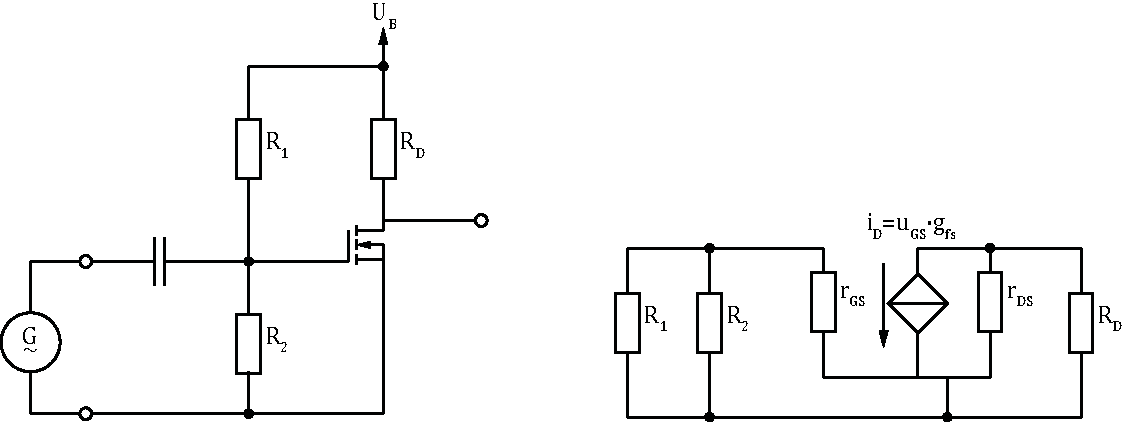
\includegraphics[width = \linewidth]{../fig/fet_source.pdf}
	\caption{Source Schaltung und Kleinsignalersatzschaltung}
	\label{fet:sourceschaltung}
\end{figure}
\noindent
Arbeitspunkteinstellung:
\[ U_{AP} = U_B - \frac{U_B - u_{DSmin}}{2} \]
\begin{tabular}{@{}ll}
  $U_B$:        & Quellenspannung
\end{tabular}
\\\\
Spannungsverstärkung:
\[ V_u = -g_{fs} \cdot (R_D || r_{DS} || R_L) \stackrel{R_L \to \infty}{=} 
-g_{fs} \cdot \frac{R_D \cdot r_{DS}}{R_D + r_{DS}} \]
Ausgangswiderstand:
\[ r_a = \frac{R_D \cdot r_{DS}}{R_D + r_{DS}} \]
Eingangswiderstand:
\[ r_e = \frac{r_{GS} \cdot R_G'}{r_{GS} + R_G'}\]
\[ R_G' = R_1 \parallel R_2 \]
